


\chapter{Fortgeschrittene Skalierungsmethoden}
%Kollege Hase Otter ich muss Abbreviations richtig in LaTeX deklarieren 
\section{Convolutional Neural Networks / Deep learning}
    \subsection{Grundlagen von Convolutional Neural Networks (CNNs)}
        Convolutional Neural Networks \ac{CNN} sind eine Art von Deep-Learning-Modell, welches besonders im Hinblick auf die Verarbeitung von Daten mit räumlicher Struktur den aktuellen Stand der Technik darstellt.      
        Räumliche Daten, wie z.B.      Bilder können bearbeitet, verarbeitet, erstellt und hauptsächlich analysiert werden.      
        CNNs bestehen aus mehreren Schichten von Neuronen, die so angeordnet sind, dass sie Merkmale extrahieren und Objekte Klassifizieren können.
        Die grundlegende Idee hinter CNNs ist die Verwendung von Faltung (engl.      convolution) zur Merkmalsextraktion und pooling layers.      
        Diese Art der Verbindung spart Rechenleistung und ermöglicht eine effektivere sowie schnellere Verarbeitung von großen Datensätzen\footfullcite{Li2022}.
        \footfullcite{kolbentwicklung,oshea2015introduction}
    \subsection{Architekturen von CNNs}
    
        Es gibt mehrere bekannte Architekturen von CNNs, darunter AlexNet\footfullcite{Aloysius2017}, ResNet\footfullcite{Pengcheng2020} und Inception\footfullcite{Zahangir2017}.

        \begin{figure}[h]
            \centering
            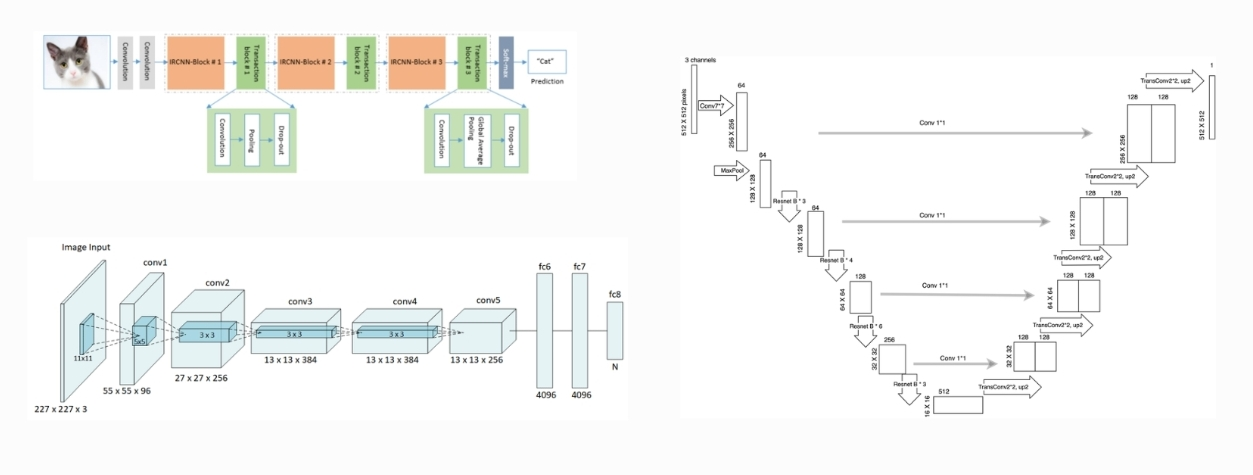
\includegraphics[width=0.8\textwidth]{img/different_types_of_cnn_nets.jpg}
            \caption{Verschiedene Architekturen von Image Networks. Oben links vereinfachtest Alex net, unten links inception net, rechts Abbildung der Res net Architektur.}
            \label{fig:my_label}
        \end{figure}
        
        AlexNet\footfullcite{Aloysius2017} war das erste CNN, das auf einem großen Datensatz erfolgreich angewendet wurde.
        ResNet zeichnet sich durch seine Fähigkeit aus, sehr tiefe Netzwerke zu trainieren, ohne dass das Problem des Verschwindens des Gradienten auftritt\footfullcite{Pengcheng2020}.  
        Inception wiederum ist für seine Fähigkeit bekannt, die Effizienz von CNNs durch die Verwendung von sogenannten Inception-Modulen zu erhöhen\footfullcite{Zahangir2017}.
        %TODO Grafiken für die Netzwerke raussuchen (BV Vorlesung?)

    
    \subsection{Anwendungen von CNNs}
    
        CNNs haben zahlreiche Anwendungen, darunter Bildklassifizierung, Objekterkennung und Gesichtserkennung.      
        Bei der Bildklassifizierung werden Bilder automatisch in verschiedene Kategorien eingeteilt.      
        Beispielsweise können Bilder in Klassen wie Hunde, Katzen oder Autos eingeteilt werden.  
        Bei der Objekterkennung wird das Modell darauf trainiert, bestimmte Objekte in einem Bild zu erkennen, wie z.B.      Personen oder Straßenschilder.      
        Die Gesichtserkennung wird oft zur Identifikation von Personen in Sicherheitsanwendungen eingesetzt.
        \footfullcite{wu2017squeezedet,liu2015deep,jaderberg2015spatial}\footnote{\url{https://www.researchgate.net/figure/Object-detection-in-a-dense-scene_fig4_329217107}}

        \begin{figure}[h]
            \centering
            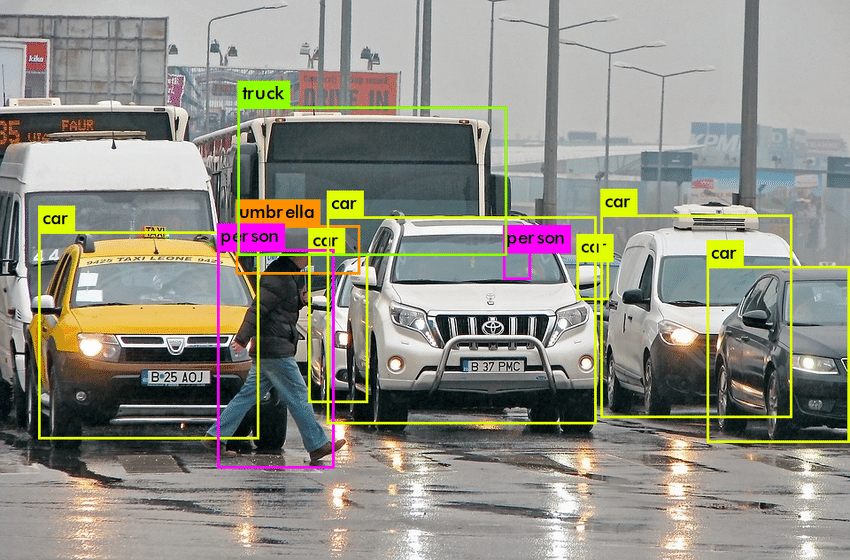
\includegraphics[width=0.6\textwidth]{img/Object-detection-in-a-dense-scene.ppm.png}
            \caption{Beispielbild eines Frames mit Bounding Boxes}
            \label{fig:Beispielbild_eines_Frames_mit_Bounding_Boxes}
        \end{figure}


    \subsection{Transfer Learning mit CNNs}
    
        Transfer Learning ist eine Technik, bei der ein bereits trainiertes CNN auf eine neue Aufgabe angewendet wird, ohne es von Grund auf neu zu trainieren.      
        Dies ist nützlich, wenn man nur über begrenzte Trainingsdaten verfügt oder wenn das Trainieren eines neuen Modells zu viel Zeit oder Ressourcen in Anspruch nimmt.      
        Ein Beispiel hierfür ist Erkennung von Autos, bei denen das Modell auf einem bereits trainierten CNN basieren kann, das auf z\.B\. Yolo v8 trainiert wurde\footfullcite{Nguyen2021}.

        In unserem Projekt haben wir das Modell resnet50 zur Trainingsgrundlage genommen, um unser eigenes Modell zu entwickeln. Wir haben den Code, den wir verwendet haben, um dieses Training durchzuführen, im Folgenden aufgeführt:

        \begin{lstlisting}
Net = torchvision.models.segmentation.deeplabv3_resnet50(pretrained=True)
        \end{lstlisting}

        Dieser Code\footnote{\url{https://github.com/studienarbeit-cnn-dhbwka-2022/Segmentation_cnn/blob/main/cnn.ipynb}} ermöglichte es uns, die Leistungsfähigkeit von resnet50 auszunutzen und es an unsere spezifischen Anforderungen anzupassen. Durch das Training unseres Modells konnten wir die gewünschten Ergebnisse erzielen und wichtige Erkenntnisse gewinnen, ohne ein Model von Grund auf zu trainieren.
        
    \subsection{Limitationen von CNNs und aktuelle Forschungsziele}

        Obwohl CNNs sehr erfolgreich bei der Verarbeitung von Bildern sind, haben sie auch einige Limitationen.      
        Zum Beispiel sind sie nicht gut geeignet, um komplexe Abhängigkeiten zwischen verschiedenen Eingabemerkmalen zu erfassen, wie z.B. das Verhalten von Objekten in einem Video.
        Zudem benötigen CNNs weiterhin viel Rechenleistung und Ressourcen
        \footfullcite{li2018visualizing}

        Facebooks Segment Anything Model (SAM) ist ein neues und Open-Source Modell, das sowohl interaktive als auch automatische Segmentierung durchführen kann.
        Die Benutzeroberfläche des Modells ermöglicht es, es auf flexible Weise zu verwenden, was eine Vielzahl von Segmentierungsaufgaben durch einfache Ingenieursarbeiten möglich macht.
        Das Modell wurde auf einem Datensatz von 11 Millionen Bildern und 1,1 Milliarden Masken trainiert und hat eine starke Null-Schuss-Leistung bei einer Vielzahl von Segmentierungsaufgaben\footnote{\url{https://research.facebook.com/publications/segment-anything/}}.

        \begin{figure}[h]
            \centering
            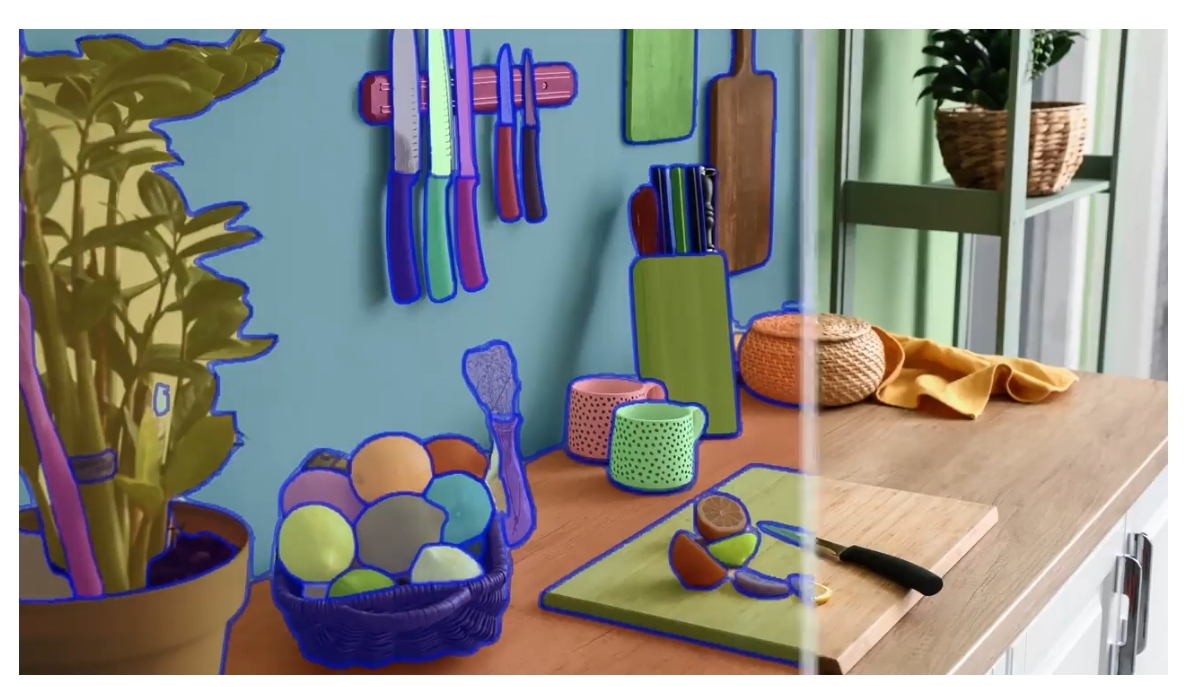
\includegraphics[width=0.6\textwidth]{img/SmartSelect_20230517_135035_Firefox.jpg}
            \caption{SAM: A generalized approach to segmentation}
            \label{fig:facebook_sam}
        \end{figure}

\section{Super Resolution}
    \subsection{Grundlagen von Super Resolution }
    
        Super Resolution \ac{SR} ist eine Technik, um aus einer niedrig aufgelösten Eingabe ein hochauflösendes Bild zu generieren.      
        Dies wird oft als Upscaling bezeichnet und findet in vielen Anwendungen wie der Bildrekonstruktion und Videoanalyse Anwendung.
        Die Grundidee hinter SR ist, dass hochauflösende Informationen in einem niedrig aufgelösten Bild versteckt sein können.      
        Die Herausforderung besteht darin, diese Informationen zu extrahieren und in ein hochauflösendes Bild zu integrieren.      
        SR ist somit ein Problem der inversen Bildgebung, bei dem eine hohe Auflösung aus einer niedrigen Auflösung abgeleitet werden muss.
        \footfullcite{7115171}
        
    \subsection{Super Resolution-Methoden auf Basis von Deep Learning}
    
        Super Resolution-Methoden auf Basis von Deep Learning haben in den letzten Jahren viel Aufmerksamkeit erhalten und sind derzeit der Stand der Technik für SR.      
        Diese Methoden verwenden Convolutional Neural Networks (CNNs) zur Verarbeitung von Bildern und zur Generierung von hochauflösenden Bildern.
        Es gibt verschiedene Arten von SR-Methoden auf Basis von Deep Learning, darunter Single-Image Super Resolution (SISR) und Multi-Image Super Resolution (MISR).      
        SISR-Methoden verwenden nur ein niedrig aufgelöstes Bild als Eingabe, während MISR-Methoden mehrere Bilder verwenden, um ein hochauflösendes Bild zu generieren.

        \begin{figure}[h]
            \centering
            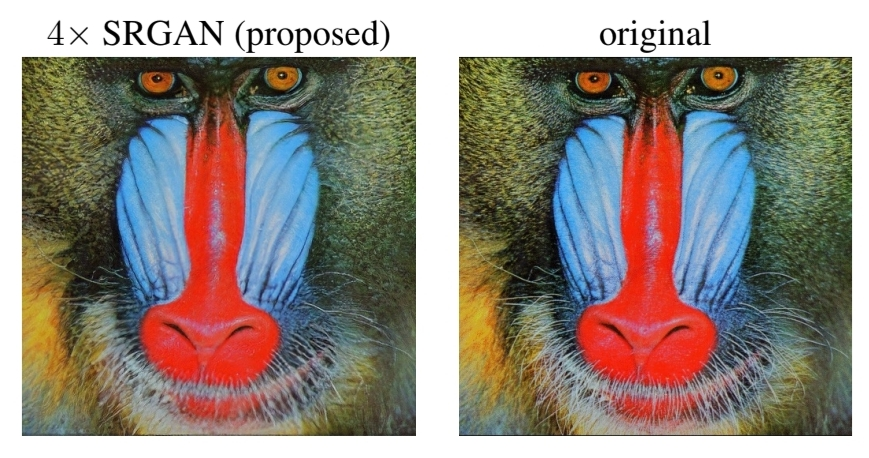
\includegraphics[width=0.7\textwidth]{img/SmartSelect_20230517_140120_Samsung Notes.jpg}
            \caption{Super resolution links, original rechts}
            \label{fig:superresolution}
        \end{figure}
        
        %TODO mehr auf sisr und misr eingehen hab ich aber nur semi verstanden so far 
    
    \subsubsection{Anwendungen von SR}
    
        SR hat viele Anwendungen in der Bild- und Videoanalyse, einschließlich der Rekonstruktion von Bildern aus medizinischen Scans, der Verbesserung von Bildern für die forensische Analyse\footfullcite{10.1007/978-0-387-73742-3_20} und der Verbesserung von Bildern für die Erkennung von Gesichtern und Objekten.
        In der Videoanalyse kann SR verwendet werden, um Videos zu stabilisieren, indem Bewegungsunschärfe reduziert und die Schärfe der Bilder verbessert wird.      
        SR kann auch bei der Entschlüsselung von unscharfen und verschwommenen Bildern in Überwachungsaufnahmen helfen.
    
    \subsubsection{Evaluierung von SR-Methoden}
    
        Die Evaluierung von SR-Methoden ist eine wichtige Aufgabe, um die Qualität und Effektivität der generierten Bilder zu bestimmen.      
        Die gängigen Evaluierungsmethoden umfassen die Verwendung von visuellen Qualitätsmetriken wie Peak Signal-to-Noise Ratio (PSNR) und Structural Similarity Index Measure (SSIM).
        Es gibt auch speziellere Evaluierungsmethoden wie die Verwendung von Perceptual Quality Assessment (PQA)-Maßnahmen, die menschliche Wahrnehmungseigenschaften berücksichtigen, um die Qualität der generierten Bilder zu bestimmen.
    
    \subsubsection{Herausforderungen und zukünftige Forschungsziele von Super Resolution}
    
        Obwohl SR-Methoden auf Basis von Deep Learning vielversprechende Ergebnisse erzielt haben, gibt es immer noch Herausforderungen und zukünftige Forschungsziele, die erforscht werden müssen.
        Eine der Herausforderungen besteht darin, dass SR-Methoden häufig dazu neigen, Artefakte in den generierten Bildern zu erzeugen, insbesondere bei der Verwendung von sehr hohen Upscaling-Faktoren.      %TODO Beispielbild Artefakte erklären
        Dies kann die visuelle Qualität der generierten Bilder beeinträchtigen und die Anwendbarkeit von SR-Methoden in bestimmten Szenarien einschränken.
        
        Eine weitere Herausforderung besteht darin, dass SR-Methoden häufig sehr rechenaufwändig sind, insbesondere wenn sie auf großen Datensätzen oder in Echtzeit angewendet werden müssen.      
        Die benötigten Ressourcen sind teuer.
        Dies kann die praktische Anwendbarkeit von SR-Methoden in einigen Anwendungen einschränken.        
        Zukünftige Forschungsziele könnten sich darauf konzentrieren, diese Herausforderungen zu überwinden, indem sie neue SR-Methoden entwickeln, die sowohl effektiv als auch effgizient sind.      
        Eine mögliche Lösung wäre die Verwendung von Generative Adversarial Networks (GANs) zur Verbesserung der visuellen Qualität der generierten Bilder und zur Reduzierung von Artefakten.      %TODO näher auf GAN eingehen 
        Eine weitere mögliche Lösung wäre die Entwicklung von neuartigen Architekturen von Deep Learning-Netzwerken, die weniger rechenaufwändig sind und schneller ausgeführt werden können\footfullcite{dong2016accelerating}\footfullcite{Park2020}.

        \subsubsection{Deep Learning Super Sampling}

        Eine vielversprechende Lösung zur Beschleunigung von Deep Learning ist Nvidia's DLSS-3 (Deep Learning Super Sampling 3, Stand 2023 Mai 17)\footnote{\url{https://www.nvidia.com/en-us/geforce/news/dlss3-ai-powered-neural-graphics-innovations/}}. 
        DLSS ist eine fortschrittliche Technologie, die von NVIDIA entwickelt wurde und es ermöglicht, hochauflösende Grafiken in Echtzeit zu rendern, indem es auf KI-Methoden basiert und durch Hardware (GPU) beschleunigt wird.
        DLSS bietet nicht nur schnellere Renderzeiten, sondern ermöglicht auch eine verbesserte Leistung auf Grafikkarten, da weniger rechenintensive Berechnungen erforderlich sind.
        Durch extensive Nutzung der CUDA cores, welche immer imposanter in Grafikarten eingebaut werden, ist das berechnen von Hohchauflösenden Bilder schneller mit jeder generation.
            
        % I want a tea party with Y'ha-nthlei

        ~
        
        Insgesamt bleibt SR ein aktives Forschungsfeld mit großem Potenzial für Anwendungen in der Bild- und Videoanalyse.      
        Mit weiteren Fortschritten in der Forschung können SR-Methoden immer leistungsfähiger und praktischer werden, um die Bedürfnisse der Industrie und der Geselllschaft zu erfüllen.

\section{Generative Adversarial Networks (GANs)}

    \subsection{Grundlagen von Generative Adversarial Networks (GANs)}
        
        Generative Adversarial Networks (GANs) sind ein leistungsstarkes Framework für das Training von Deep Learning-Modellen zur Generierung von Daten.      
        GANs bestehen aus zwei miteinander konkurrierenden neuronalen Netzwerken, einem Generator und einem Diskriminator.

        \begin{figure}[h]
            \centering
            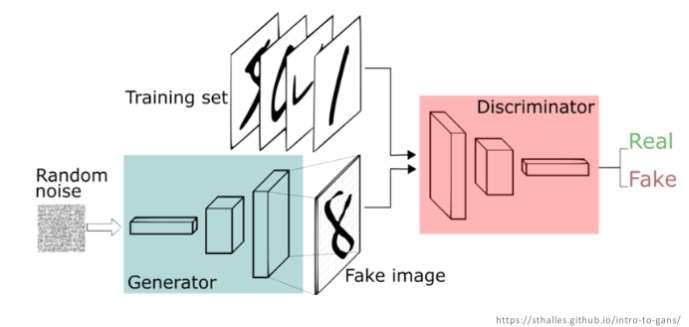
\includegraphics[width=0.7\textwidth]{img/GAN_architecture.jpg}
            \caption{Der Generator erzeugt neue Daten, während der Diskriminator versucht, zwischen den vom Generator erzeugten Daten und den echten Daten zu unterscheiden.}
            \label{fig:GAN_aufbau}
        \end{figure}
        
        Im Laufe des Trainings passt sich der Generator kontinuierlich an und verbessert seine Fähigkeit, realistische Daten zu generieren, während der Diskriminator gleichzeitig verbessert wird, um zwischen den generierten und echten Daten zu unterscheiden.
        %TODO GRAFIK! LUKAS! GRAFIK!
    
    \subsection{Architekturen von GANs}
    
        Es gibt verschiedene Architekturen von GANs, die für verschiedene Arten von Anwendungen geeignet sind.      
        in Beispiel ist das Deep Convolutional GAN (DCGAN), das speziell für die Generierung von Bildern entwickelt wurde.      %TODO Bild? ALso so architekkturbild oder so idk
        DCGAN nutzt Convolutional Neural Networks (CNNs) und Transposed Convolutional Neural Networks, um Bilder zu generieren, die visuell realistisch aussehen und strukturell konsistent sind.
        Ein weiteres Beispiel ist das CycleGAN\footfullcite{CycleGAN2017}, das für die Bildübersetzung zwischen verschiedenen Domänen verwendet werden kann.      
        CycleGAN nutzt einen Generator und einen Diskriminator sowie zusätzliche Cycle-Verlustfunktionen, um die Transformationen zwischen den Bildern in verschiedenen Domänen zu erlernen.%todo quellen vergessen
    
    \subsection{Anwendungen von GANs}
    
        GANs finden Anwendungen in verschiedenen Bereichen wie der Bildgenerierung, Style Transfer, der Verbesserung von Bildern und der Videoanalyse.      
        Zum Beispiel können GANs verwendet werden, um realistisch aussehende Bilder von Gesichtern, Landschaften oder anderen Objekten zu generieren.

        \begin{figure}[h]
            \centering
            
\includegraphics[width=0.4\textwidth]{img/cactus.jpg}
            \caption{Eingabe in das Modell: A small cactus wearing a straw hat and neon sunglasses in the Sahara desert.: \url{https://imagen.research.google/}}
            \label{fig:GAN_example}
        \end{figure}


        Style Transfer ermöglicht die Veränderung des visuellen Erscheinungsbildes von Bildern durch die Übertragung des Stils von einem Bild auf ein anderes.
        Dabei wird ein vortrainiertes neuronales Netzwerk verwendet, um Merkmale des Stils und Inhalts eines Bildes zu erfassen und zu kombinieren.
        Diese Technik hat Anwendungen in der Bildbearbeitung, Kunstgenerierung und visuellen Effekterstellung gefunden.
        
        Durch Style Transfer kann der visuelle Stil eines Bildes auf ein anderes übertragen werden, wobei ein vortrainiertes neuronales Netzwerk die Merkmale des Stils und Inhalts erfasst.
        Dies ermöglicht künstlerische Effekte und Anpassungen in der Bildbearbeitung und eröffnet neue Möglichkeiten für die kreative Gestaltung von visuellen Inhalten.

        Wie im dargestellten Bild zu sehen ist, wird das ursprüngliche Bild mithilfe des Stils des Gemäldes übertragen, wobei die Konturen des Hundes weiterhin erkennbar bleiben.

        \begin{figure}[h]
            \centering
            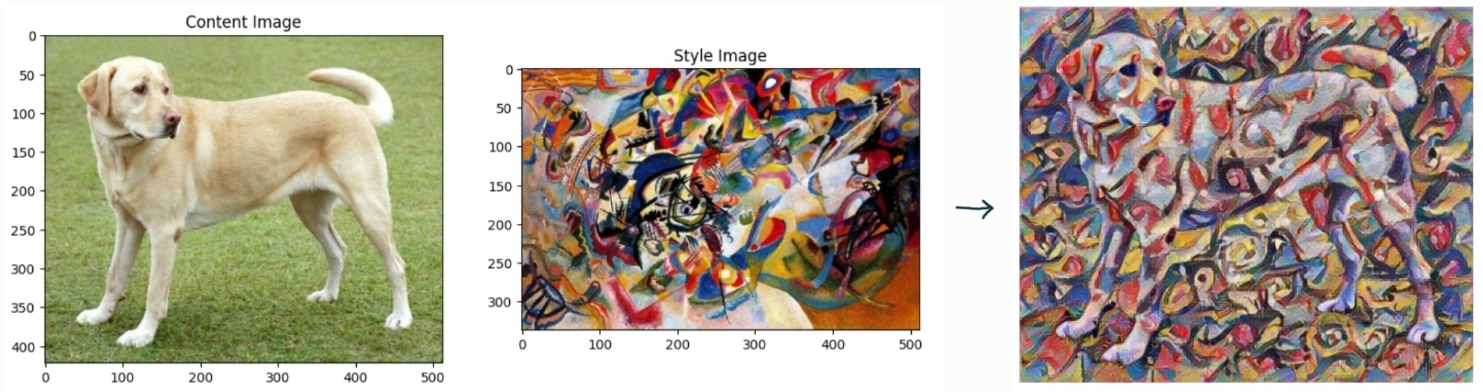
\includegraphics[width=0.9\textwidth]{img/GAN_style_trtansfer.jpg}
            \caption{\url{https://www.tensorflow.org/tutorials/generative/style_transfer}}
            \label{fig:GAN_style_transfer}
        \end{figure}
        
        GANs können auch verwendet werden, um Bilder mit höherer Auflösung oder besserer Qualität zu generieren, indem sie niedrig aufgelöste Bilder als Eingabe verwenden.
        GANs werden immer öfters in Bildverabreitungstools eingesetzt um fehlende Bereiche zu füllen, oder zum erweitern von Bildern (siehe \ref{fig:extend_image_imagen})\footnote{\url{https://imagen.research.google/}}.

        \begin{figure}[!h]
          \centering
          \begin{minipage}[b]{0.6\textwidth}
            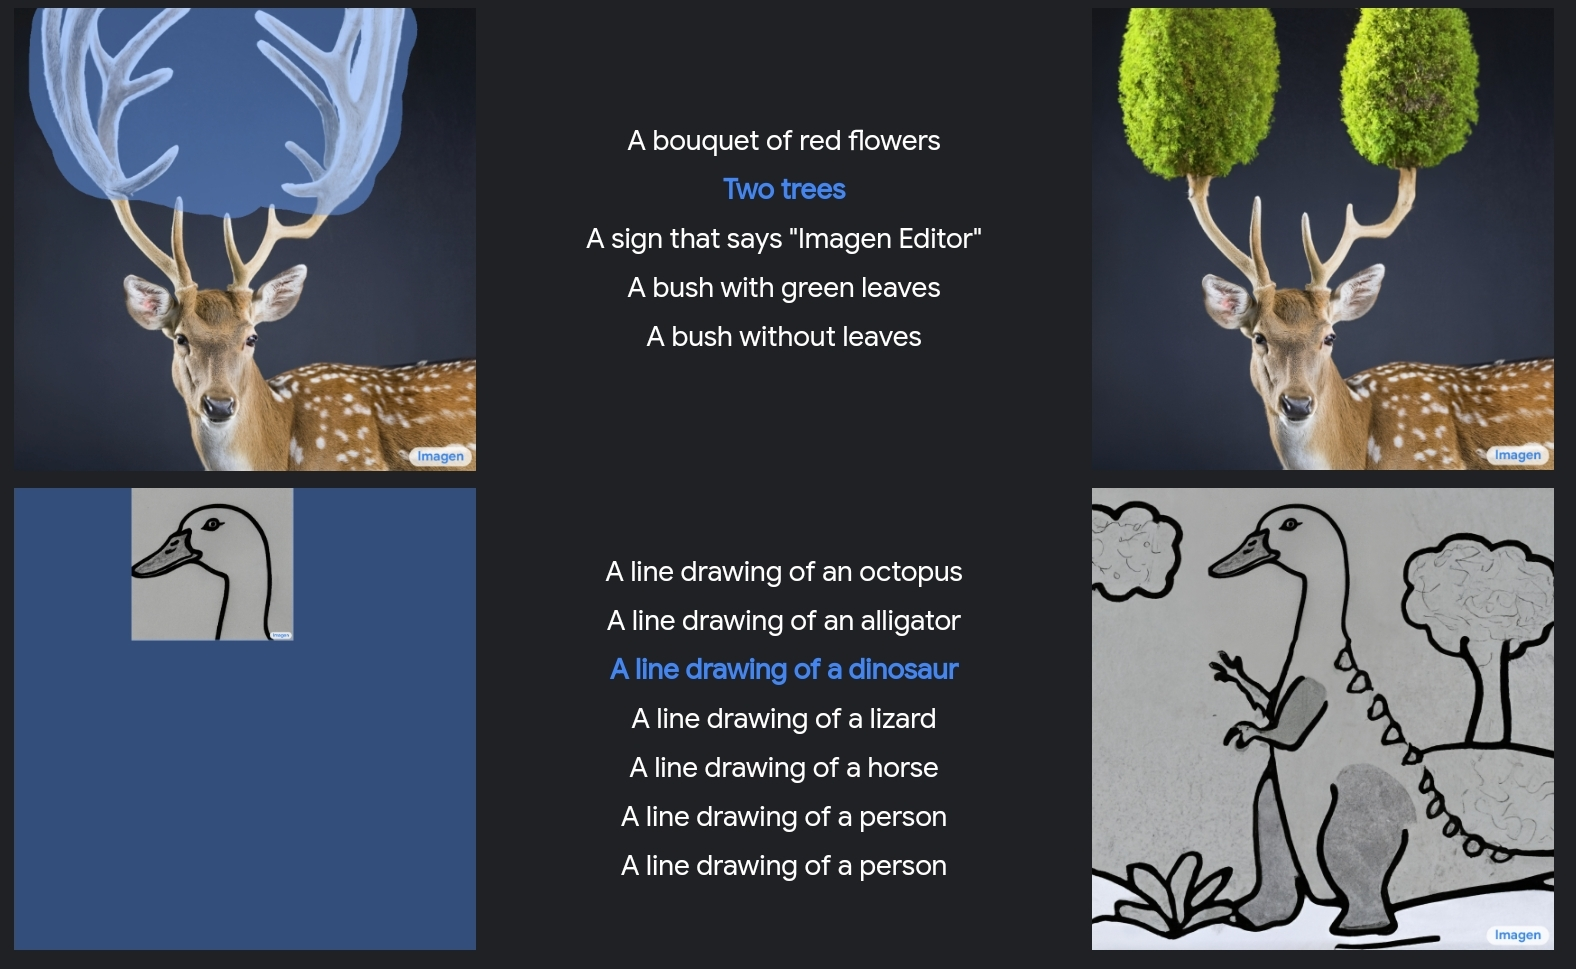
\includegraphics[width=\textwidth]{img/imagen_google_fill_and_extend.jpg}
          \end{minipage}
          \hfill
          \begin{minipage}[b]{0.35\textwidth}
            \caption{Füllen von markierten Bereichen eines Bildes durch verwendung von Imagen und Erweitern von Bildern mithilfe von Imagen, Google.}
          \end{minipage}
          \label{fig:extend_image_imagen}
        \end{figure}

        \newpage 
        % I cant deal with stupid latex anymore. Icant ocant icant

        In der Forschung können GANs verwendet werden, um Videosequenzen zu generieren oder zu verbessern. Ein modernes beispiel wäre Facebooks errungenschaften durch Make-A-Video\footnote{\url{https://ai.facebook.com/blog/generative-ai-text-to-video/}}, siehe \ref{fig:facebook_make_a_video}.

        \begin{figure}[!h]
            \centering
            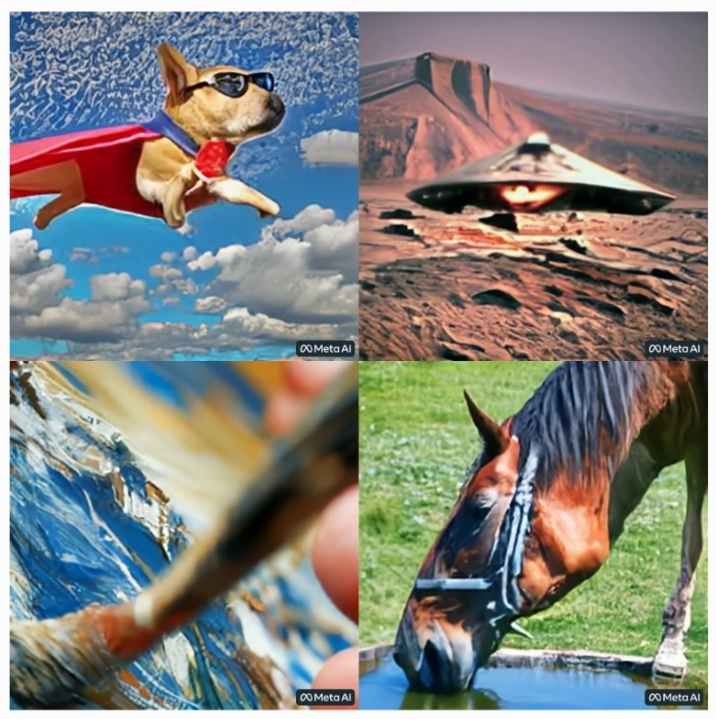
\includegraphics[width=0.6\textwidth]{img/facebook_make_a_video.jpg}
            \caption{Generierung kurzer Videos, anhand von sehr einfachen Beschreibungen.}
            \label{fig:facebook_make_a_video}
        \end{figure}
        
        Da wir leider nicht in Hogwards leben\footnote{Interaktive Zeitung aus Harry Potter: \url{https://youtu.be/xaBEFqFVSE8}}, können Videos \textit{nicht} auf PDFs angezeigt werden, noch weniger auf Papier. Die Eingaben für das Modell sind wie folgt: 
        Oben Links: A dog wearing a superhero cape flying through the sky.
        Oben rechts: A spaceship landing on Mars.
        Unten links: An artist's brush painting on a canvas close up, highly detailed. 
        Unten rechts: A horse drinking water.
        

    \subsection{Training von GANs und Evaluierung von generierten Ergebnissen}

        Das Training von GANs ist eine Herausforderung, da es sich um ein adversariales Lernverfahren handelt.      
        Das bedeutet, dass es zwei Netze gibt, die sich gegenseitig trainieren und verbessern.      %TODO Grafik & Quellen
        % Nö

        ~
        
        Das generative Netzwerk versucht, Bilder zu erzeugen, die von einem diskriminierenden Netzwerk nicht von echten Bildern unterschieden werden können.      
        Das diskriminierende Netzwerk wird trainiert, um echte Bilder von den vom generativen Netzwerk generierten Bildern zu unterscheiden.
        Das Training von GANs erfolgt durch die Minimierung einer Verlustfunktion, die als GAN-Verlust bezeichnet wird.

        ~
        
        Der GAN-Verlust besteht aus zwei Komponenten: dem Verlust des generativen Netzes und dem Verlust des diskriminierenden Netzes.      
        Der Verlust des generativen Netzes wird minimiert, wenn dasd Netzwerk Bilder erzeugt, die vom diskriminierenden Netzwerk nicht als gefälscht erkannt werden.      
        Der Verlust des diskriminierenden Netzes wird minimiert, wenn das Netzwerk in der Lage ist, besonders zuverlässig und schnell zwischen echten und generierten Bildern zu unterscheiden.
        Die Evaluierung von generierten Ergebnissen ist eine wichtige Aufgabe bei der Arbeit mit GANs.

~

        Es gibt verschiedene Methoden zur Bewertung von GANs, wie beispielsweise die visuelle Bewertung, die qualitative Bewertung und die quantitative Bewertung.  
        Die visuelle Bewertung beinhaltet das Betrachten der generierten Bilder, um zu beurteilen, ob sie realistisch aussehen oder nicht.      
        Die qualitative Bewertung beinhaltet die Verwendung von Bewertungsskalen, um die Qualität der generierten Bilder zu bewerten.      
        Die quantitative Bewertung beinhaltet die Verwendung von Metriken wie der Inception Score oder der Frechet Inception Distance, um die Qualität der generierten Bilder zu bewerten.

    \subsection{Ethische und soziale Implikationen von GANs}

    \begin{center}
        \textit{There are several ethical challenges facing text-to-image research broadly. We offer a more detailed exploration of these challenges in our paper and offer a summarized version here. First, downstream applications of text-to-image models are varied and may impact society in complex ways.}

        \url{https://imagen.research.google/}
    \end{center}
    
        Obwohl GANs eine vielversprechende Technologie sind, gibt es auch ethische und soziale Implikationen, die berücksichtigt werden müssen.      
        Ein Problem bei der Verwendung von GANs ist, dass sie zur Erzeugung gefälschter Bilder oder Videos verwendet werden können.      
        Dies kann zu Fälschungen und Manipulationen führen, die negative Auswirkungen auf die Gesellschaft haben können.
        Auch Rufschädigung kann durch GANs errleichtert werden.
        Ein weiteres Problem bei der Verwendung von GANs ist, dass sie möglicherweise nicht fair sind.  

        ~

        GANs können aufgrund ihrer Lernmethode unbewusste Vorurteile aufnehmen und in ihren generierten Ergebnissen widerspiegeln.      
        Dies kann zu diskriminierenden Ergebnissen führen, die unfaire Entscheidungen unterstützen.
        Es ist wichtig, dass bei der Verwendung von GANs Ethik und soziale Verantwortung berücksichtigt werden.      
        Es sollten Maßnahmen ergriffen werden, um sicherzustellen, dass GANs fair und ethisch korrekt arbeiten.      
        Zum Beispiel können spezielle Algorithmen entwickelt werden, um unbewusste Vorurteile zu minimieren.      
        Weiterhin können Regierungsbehörden und andere Organisationen Maßnahmen ergreifen, um den Missbrauch von GANs zu verhindern.   
        Das finden eines Kompromiss aus Forschung und politischer Einschränkung übersteigt jedoch den Rahmen dieser Arbeit.      
    
\section{Multiscale-Skalierung}

    In vielen Anwendungen der Bildverarbeitung und Computergrafik ist es notwendig, Objekte oder Strukturen in verschiedenen Größenordnungen zu analysieren oder darzustellen.      
    Multiscale-Skalierung bezeichnet Techniken und Vorgehen, die es ermöglichen, Objekte oder Signale auf verschiedenen Skalen zu untersuchen oder zu manipulieren.      
    Dabei können sowohl lokale als auch globale Eigenschaften eines Objekts berücksichtigt werden.
    Diese Möglichkeiten komplementieren häufig Implementierungen von künstlichen Intelligenzen
    %TODO Zitat richtig einbauen

    \begin{center}
        \textit{Machine learning and multiscale modeling mutually complement one another.}\footfullcite{alber2019integrating}
    \end{center}
    
    \subsection{Grundlagen von Multiscale-Skalierung}
    
        Multiscale-Skalierung ist ein Konzept aus der Signal- und Bildverarbeitung, das auf der Idee basiert, dass Signale und Bilder aus verschiedenen Skalen von Strukturen aufgebaut sind.
        In der Praxis bedeutet dies, dass ein Signal oder Bild auf verschiedene Skalen abgetastet oder transformiert wird, um Informationen auf verschiedenen Größenskalen zu erhalten.
        Ein grundlegendes Konzept der Multiscale-Skalierung ist die Skaleninvarianz.      
        Das bedeutet, dass die Informationen in einem Signal oder Bild unabhängig von der Skala erhalten bleiben sollten.      
        Das heißt, dass dieselben Merkmale oder Strukturen auf verschiedenen Skalen erkennbar sein sollten.
        \footfullcite{mallat1989theory,huang2017densely}
    
    \subsection{Methoden zur Multiskalenanalyse}
    
        Es gibt verschiedene Techniken zur Multiskalenanalyse, darunter Wavelet-Transformation und pyramidenartige Strukturen.      
        Wavelet-Transformation ist eine Methode zur Analyse und Synthese von Signalen oder Bildern auf verschiedenen Skalen.      
        Dabei wird das Signal oder Bild auf verschiedene Skalen und Frequenzen zerlegt, um Informationen auf verschiedenen Skalen zu erhalten.
        Pyramidenartige Strukturen sind eine weitere Methode zur Multiskalenanalyse, die in der Bildverarbeitung häufig verwendet wird.      
        Dabei wird das Signal oder Bild auf verschiedenen Skalen durch wiederholte Subsampling- und Filterungsoperationen reduziert.      
        Auf jeder Ebene der Pyramide wird das Signal oder Bild auf eine kleinere Größe reduziert, um Informationen auf verschiedenen Skalen zu erhalten.
        \footfullcite{burt1987laplacian,nah2017deep}
    
    \subsection{Methoden zur Multiskalenanalyse}
        Es gibt verschiedene Methoden zur Multiskalenanalyse, darunter Wavelets und Pyramiden.      
        Wavelets basieren auf der Zerlegung von Signalen in unterschiedliche Frequenzbänder, wodurch eine Multiskalenanalyse ermöglicht wird.      
        Eine Wavelet-Transformation kann auf ein Signal angewendet werden, um es in seine Hoch- und Niederfrequenzkomponenten zu zerlegen.      
        Diese Komponenten können dann unabhängig voneinander verarbeitet werden, um eine Analyse auf verschiedenen Skalen durchzuführen.
        Pyramiden sind eine weitere Methode zur Multiskalenanalyse, die auf der Idee der rekursiven Unterteilung von Signalen in immer feinere Skalen basiert.      Dabei wird ein Signal in eine Pyramide aus verschiedenen Ebenen unterteilt, wobei jede Ebene eine andere Skala darstellt.      
        Die unterste Ebene enthält das Originalsignal, während die oberen Ebenen eine immer gröbere Approximation des Signals enthalten.
        \footfullcite{simoncelli1996noise}
    
    \subsection{Anwendungen von Multiscale-Skalierung}
        Multiscale-Skalierung hat viele Anwendungen in der Bildverarbeitung und Computer Vision.
        Ein Beispiel ist die Texturanalyse, bei der Texturen auf verschiedenen Skalen analysiert werden, um Muster und Strukturen zu identifizieren.      
        Multiscale-Skalierung wird auch in der Bildkompression verwendet, um Bilder auf verschiedene Auflösungen zu skalieren und so Speicherplatz zu sparen.
        In jüngerer Zeit wurde die Multiskalenanalyse auch in Verbindung mit Deep Learning eingesetzt, um Modelle zu entwickeln, die auf verschiedenen Skalen arbeiten können.      
        Ein Beispiel ist das Multiscale Dense Network \ac{MSDN}, das eine skalierbare Architektur für die Bilderkennung bietet, die auf mehreren Skalen arbeiten kann.
    
    \subsection{Limitationen und zukünftige Forschungsziele von Multiscale-Skalierung}
        Obwohl die Multiskalenanalyse in vielen Bereichen der Bildverarbeitung und Computer Vision erfolgreich eingesetzt wurde, gibt es auch einige Limitationen.  
        Eines der Hauptprobleme ist die Herausforderung, die richtige Skala für eine bestimmte Aufgabe zu wählen.      

        
        In einigen Fällen kann dies schwierig sein, da verschiedene Skalen unterschiedliche Informationen enthalten.
        Eine weitere Herausforderung besteht darin, die Multiskalenanalyse mit Deep Learning-Methoden zu integrieren.      
        Während einige Fortschritte in diesem Bereich gemacht wurden, gibt es immer noch Raum für Verbesserungen, um die Multiskalenanalyse nahtlos in Deep Learning-Architekturen zu integrieren\footfullcite{he2016deep}.
        
        Zukünftige Forschungsrichtungen könnten sich auf die Entwicklung von verbesserten Methoden zur Skalierung und Multiskalenanalyse konzentrieren, die eine höhere Genauigkeit und Effizienz ermöglichen.      
        Darüber hinaus könnten Forscher daran arbeiten, die Integration der Multiskalenanalyse in Deep Learning-Architekturen weiter zu verbessern, um noch bessere Ergebnisse zu erzielen.

\section{Vor- und Nachteile der fortgeschrittenen Methoden}

    Im Hinblick auf die Bildqualität sind Deep-Learning-basierte Methoden wie Super Resolution und GANs den traditionellen Methoden wie der Bilinear-Interpolation überlegen.      
    Diese Methoden können hochwertige Bilder mit hoher Auflösung und Details erzeugen, die den Originalbildern nahe kommen.      
    Insbesondere die GANs erlauben die Erzeugung von realistisch aussehenden Bildern, die schwer von echten Bildern zu unterscheiden sind.
    Ein weiterer Vorteil der fortgeschrittenen Methoden ist ihre Fähigkeit zur Generierung von neuen Inhalten.   
    So können GANs und Style Transfer genutzt werden, um neue Bilder zu erzeugen, die auf den Stil und Inhalt anderer Bilder basieren.      
    Dies bietet neue kreative Möglichkeiten in der Kunst und Design.

    Jedoch stellen diese fortgeschrittene Methoden auch Herausforderungen bei der Anwendung dar.      
    Beispielsweise benötigen Deep-Learning-Methoden große Datensätze und Rechenleistung, um optimal zu funktionieren\footfullcite{li2021beginner}.      
    Ein weiteres Problem ist die Interpretierbarkeit\footfullcite{he2023segmentation} der Ergebnisse, da es schwierig sein kann, zu verstehen, wie ein Modell zu seinen Ergebnissen gekommen ist.
    Die Anwendung von fortgeschrittenen Skalierungsmethoden hat auch Auswirkungen auf die Leistung und Effizienz von Systemen\footfullcite{Wang2018}.      
    So können Deep-Learning-basierte Methoden in Echtzeit-Anwendungen, wie beispielsweise autonomen Fahrzeugen, zu Verzögerungen führen.      
    Es ist daher wichtig, dass die Anforderungen an Leistung und Effizienz bei der Auswahl der Skalierungsmethode berücksichtigt werden.
    
    Es gibt moderne Architekturen und Techniken für höchst effiziente und leistungsstarke Ergebnisse.
    Zukunftsaussichten für fortgeschrittene Skalierungsmethoden liegen in der Kombination verschiedener Methoden. 
    So können beispielsweise GANs und Super Resolution zusammen genutzt werden, um qualitativ hochwertige und realistisch aussehende Bilder zu erzeugen.      
    Ein weiteres Forschungsgebiet ist die Verbesserung der Interpretierbarkeit und Erklärbarkeit von Deep-Learning-Modellen.      
    
    Insgesamt bieten fortgeschrittene Skalierungsmethoden in der Bildverarbeitung und Computergrafik viele Vorteile, jedoch müssen auch die Herausforderungen bei der Anwendung und die Auswirkungen auf die Leistung und Effizienz von Systemen berücksichtigt werden\footfullcite{Klver2022}.      
    Zukünftige Forschung sollte darauf abzielen, die verschiedenen Methoden zu kombinieren und die Interpretierbarkeit von Deep-Learning-Modellen zu verbessern.

\newpage